\chapter{Experiments}
\label{chap:experiments}
% Describe the degree project. What did you actually do? This is the practical description of how the method was applied.

% %TODO -- Implementation details
% \section{Implementation}
% \subsection{Developments}
% \lipsum[1] % FIXME
% \subsection{Monitoring}
% \lipsum[1] % FIXME



\subsection{Bag of Tricks}
The techniques to improve the \ac{gan} training and the reasoning behind their importance are eloborated in papers such as \cite{soumith2017wasserstein,goodfellow2014generative,openaigan2wgan,improved_gan}. The important hacks or tricks from these papers and other sources are compiled in \cite{gan_hacks} and are wildly adapted in the field. Since the majority of the work in the field are on images, some of these tricks do not help and sometimes even hurt the training. These ticks along with the pre-processing steps mentioned in \ref{sec:preprocessing} are crutical for proper training of the network. The tricks are as follows. %TODO correct when changed to experiemnts
 
\paragraph{Normalizing Inputs} 
It is common practice to normalize the inputs before training a neural network. When it comes to \acp{gan}, the output of the generator is the input of the discriminator. Hence it is suggested to normalize the images between [-1,1] by using a Tanh activation function at the output layer of the generator. This is another motivation behind predicitng the poses in range [-1,1] and then scaling the make the upper half of the pose to unit length.

\paragraph{Modified Loss function}
The theory the generator component of the \ac{gan} loss \ref{eqn:gan_loss}, $log(1-D(G(z)))$ is minimized. As explained in \ref{subsec:gan}, it is replaced with maximizing $log(D(G(z)))$ as the former leads to vanishing gradients early on during the training. This is referred to as the $-logD$ trick. In practice the label for fakes are flipped as reals while training the generator, since the goal is to make the generator's output real according to the discriminator. And as the \ac{bce} loss \ref{eqn:loss_bce} which has a negative magnitude in its formulation is used, maximization is achieved while minimizing the loss during training. Note that the generator variable $G(z)$ in our training procedure is actually $P(Q(\textbf{x}))$. 

\paragraph{Spherical Latent Space}
Sample $z$ from a spherical distribution instead of uniform distribution. Doing interpolation along the great circle \ref{fig:great_circle} rather than a straight line from sample A to sample B. This spherical linear interpolation prevents the divergence of samples from the model's prior distribution and produces ouput with better features.

\begin{figure}[h] 
    \centering
    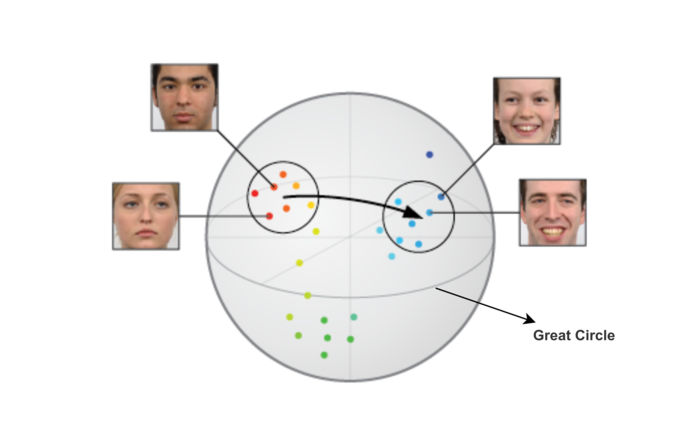
\includegraphics[width=\textwidth]{figures/background/sphericalZ.png}
    \caption{Illustration of the sampling from the great circle. Image source \cite{spherical_sampling}}
    \label{fig:great_circle}
\end{figure}

\paragraph{BatchNorm}
Training the \ac{gan} using separate batches of real and fake data without mixing them. And perform instance normalization when batch normalization is not possible.

\paragraph{Avoid Sparse Gradients}
Sparse gradients affect the trianing stability of the \ac{gan}. Hard functions like hard- \ac{relu}, Max Pooling that have sparse gradients should be avoided. Instead Leaky-\ac{relu} work well for both the generator and the discriminator. And average pooling, or convolution layers with stride are better for downsampling or upsampling.



\paragraph{Shperical Latent Space}

\subsubsection{label smooting}
more discriminator didnt work

\subsubsection{drop out}
dropout should be less for vae
